% software requirements and reasoning (8-10 pages)
\chapter{Проектиране на библиотека за създаване на текстов потребителски 
интерфейс}
\hfill

\section{Функционални изисквания}

        Изискванията, поставени върху проекта са следните:

        \begin{itemize}
                \item Подредба и структуриране на елементи на потреителски
                        инерфейс
                        \begin{itemize}
                                \item[--] Елементите трябва да имат стриктна 
                                        йерархична структура.
                                \item[--] Елементите трябва да могат да се
                                        подреждат спрямо себе си и други 
                                        компоненти.
                        \end{itemize}
                \item Елементи на потребителски интерфейс с добавена
                        функционалност
                        \begin{itemize}
                                \item[--] Трябва да има елементи, които
                                        изпълняват някаква конкретна
                                        функционалност. Те могат да бъдат:
                                        \begin{itemize}
                                                \item Етикет - елемент, който
                                                        показва текст. 
                                                \item Бутон - изпълнява
                                                        зададена функционалност
                                                        при натискане.
                                                \item Въвеждане - позволява на 
                                                        потребителя да въвежда
                                                        текст.
                                        \end{itemize}
                        \end{itemize}
                \item Обработка на събития от мишка и клавиатура
                        \begin{itemize}
                                \item[--] Приложенията, трябва да могат да
                                        отчитат и реагират на събития от 
                                        клавиатура и мишка.
                        \end{itemize}
        \end{itemize}

\section{Подбор на средства за разработка}
        \subsection{Програмен език}

                Текущата дипломна работа е реализирана на програмния език 
                Python.
                \newline

                Езикът за програмиране Python е създаден в началото на 90-те 
                години на миналия век от холандския програмист Гуидо ван Росум.
                По това време той иска да създаде лесен за изучаване език с 
                общо предназначение, който да преодолява ограниченията на езици
                като С. Поради синтактичната си близкост до английския език и 
                гореизброените причини Python бързо набира популярност. 

                Python е обектно ориентиран и строго типзиран език от високо
                ниво, като типовете на данните се определят по време на 
                изпълнението. Поради скриптовия си характер, липсата на 
                необходмиост от задаване на типа на променливи и вградените 
                сложни полиморфни типове (списъци и речници), когато сравняванo
                с други езици с общо предназначение, времето за разработка на 
                програми написани на Python е значително по-малко. Те са 3-5 
                пъти по-кратки от еквивалентите на Java и 5-10 пъти от тези на 
                C++. \cite{py-comp}
                % Comparing python to other languages - https://www.python.org/doc/essays/comparisons

                От 2003 г. насам Python се класира в топ 10 на най-популярните
                езици за програмиране. В момента на писане на дипломната работа
                е определен за най-популярен според `TIOBE Programming 
                Community Index`. Езикът намира обширна употреба, като 
                най-често се използва при анализ на данни, научни изчисления, 
                изкуствен интелект както и в сферата на информационната 
                сигурност.  \cite{TIOBE}
                % Language popularity https://www.tiobe.com/tiobe-index/

                Основните недостатъци на приложения, написани на Python, са 
                скоростта им на изпълнения и паметта, която заделят. Това не е
                проблем за текущия проект, защото скоростта е ограничена от
                бодовете на терминала, в който се изпълнява, а паметта е 
                пренебрежима за модерните комютри. 

        \subsection{Статичен анализатор}
                
                Много софтуерни проекти използват инструменти, които 
                сигнализират за грешки в програмирането, бъгове, стилистични
                грешки и подозрителни конструкции.

                Текущият проект използва \textbf{flake8} и \textbf{pylint} за
                статичен анализ на  код. И двата инструмента проверяват за
                спазването на официалното ръководство за стила на кода на
                Python (PEP8). Въпреки че се препокриват на някои места, двата
                статични анализатора проверяват и за спазването на допълните
                практики при писане на код, които се различават.
                % Python standard guide - https://peps.python.org/pep-0008/
        \subsection {Компонентно тестове}
                
                При компонентното тестване (Unit Testing) се проверява дали 
                отделни единици код (методи или класове) работят правилно. За
                разработката на текущия проект е използвана библиотеката
                \textbf{pytest}. Използвани са плъгините pytest-cov и
                pytest-asyncio за проверка на покритието на тествания код и
                съвместимост при тестване на асинхронни методи.

        \subsection{Система за управление на версиите}

                Всеки един софтуерен проект в днешно време използва някакъв вид
                система за управление на версиите. Най-разпространената такава
                система е \textbf{git}. Тя позволява проследяването на всички 
                промени по кода, като по този начин подпоага сътрудничеството 
                на големи екипи от хроа.

                По време на разработката на текущия проект бе използвана
                стратегия на разклоненията (branching strategy), при която 
                всяко изискване по проекта има свое отделно разклонение:

                \begin{itemize}
                        \item area - разработка на вътрешното растеризиране 
                                на компонентите
                        \item compositor/button - разработка на елемент 
                                'бутон'
                        \item compositor/input - разработка на елеметн 
                                'въвеждане'
                        \item compositor/label - разработка на елемент 
                                'надпис'
                        \item compositor - разработка на алгоритъм за
                                коммпозиране на елементи
                        \item events - работа със събития от периферни 
                                устройства
                        \item styles - разработка на настройки за 
                                персонализиране на елементи
                \end{itemize}

        \subsection{Непрекъсната интерграция}

                Непрекъснатата интеграция (Continuous Integration) 
                \figref{fig:ci-cd} e практика при разработката на софтуер при 
                която работата на много разработчици се обединява на едно 
                място, след което се задейства автоматизирана 
                компилация/интерпретация и тестване на софтуерния продукт.

                \begin{figure}[h]
                        \centering
                        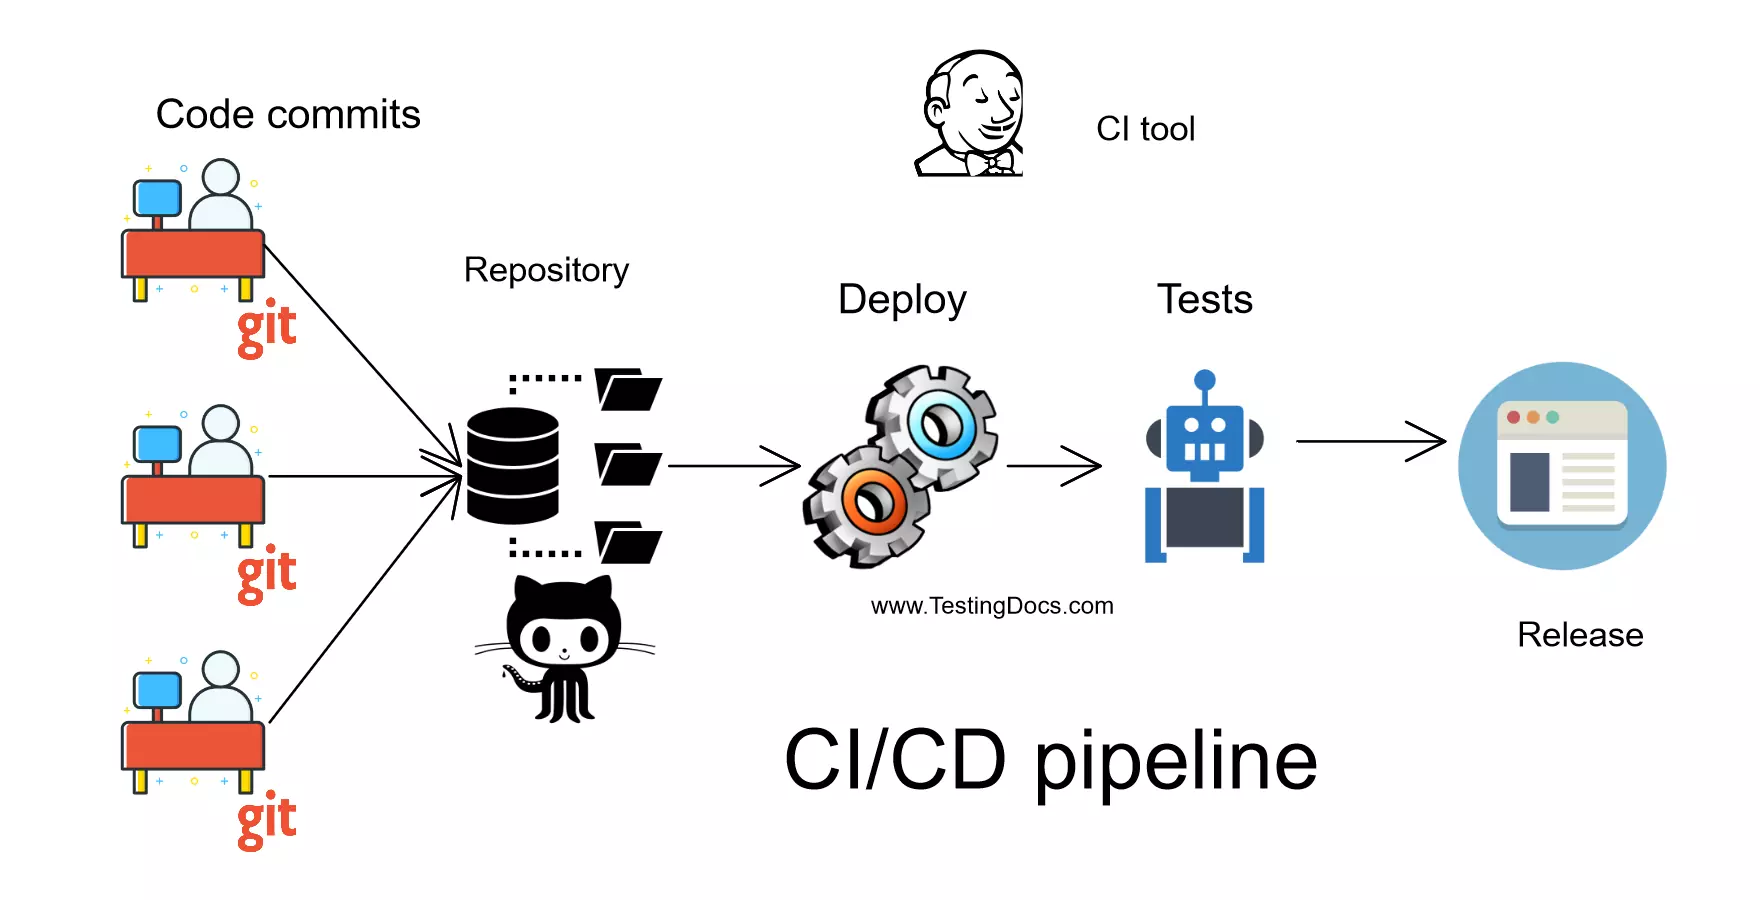
\includegraphics[width=1\textwidth]{images/ci-cd.png}
                        \caption{Непрекъсната интеграция}
                        \label{fig:ci-cd}
                \end{figure}

                По време на разработката на текущия проект бяха използвани 
                предоставените от платформата \textbf{GitHub} средства за 
                автоматизирани тестване и статичен анализ на кода (GitHub 
                Actions).

        \subsection{Среда за разработка}

                Текущата дипломна работа бе разработена на операционната
                система Arch Linux, като за редакция на кода и документацията 
                бе използвана конфигурация на текстовия редактор Neovim - 
                Astronvim. Кодът на проекта бе публикуван онлайн в платфомата 
                GitHub. Настоящата документация бе написана с помощта на 
                \LaTeX.

